\begin{savequote}[75mm]
What I cannot create, I do not understand.
\qauthor{Richard Feynman}
\end{savequote}

% pending plagiarism check
\begin{flushleft}
\chapter{Image-based Profiling of genetically engineered models of early colorectal cancer development}

\section{Motivation}

In the previous chapter I demonstrated that (1) interpretable multi-view representations from patient derived organoids can be learnt and (2) treatment-induced morphological changes can be interpreted using these multi-view representations to guide their mechanistic validation. Building on these observations, I wondered whether this approach could be extended to further understand early colorectal cancer pathogensis and identify small molecule treatments that interfere with disease-associated phenotypes. To this end I created a set of four genetically engineered mouse colon organoid lines that model the initiation of colorectal cancer by harboring tumorigenic \textit{Apc} and \textit{Kras} mutations in isolation and combination. The organoid models were then characterised using transcript expression, proteomics and lipidomics measurements. A high-throughput image-based profiling experiment covering c.a 1700 well-annotated FDA-approved, natural and targeted small molecules was performed. I then explored wether a multi-view representation model could be used to interpret treatment-induced morphologies and identify small molecules that acted specifically on phenotype changes caused by tumorigenic \textit{Apc} and \textit{Kras} mutations. 

\section{Generation and characterization of organoid models}
\subsection{Generation of organoid colon adenoma models}
The emergence of colorectal cancer via the chromosomal instability process is a well understood sequence of genetic events that start with hyperactivation of canonical Wnt signaling, i.e. through truncating mutations of \textit{Apc}, followed by the hyperactivation of ERK-MAPK signaling, i.e. via oncogenic mutations of \textit{KRAS}. I genetically engineered mouse colon organoid models carrying \textit{Apc} truncating mutations and/or a \textit{Kras}\textsuperscript{G12D} allele, thereby modelling the first set of genetic events within the chromosomal instability process leading to colorectal cancer. 

\begin{figure}[H]
\centering
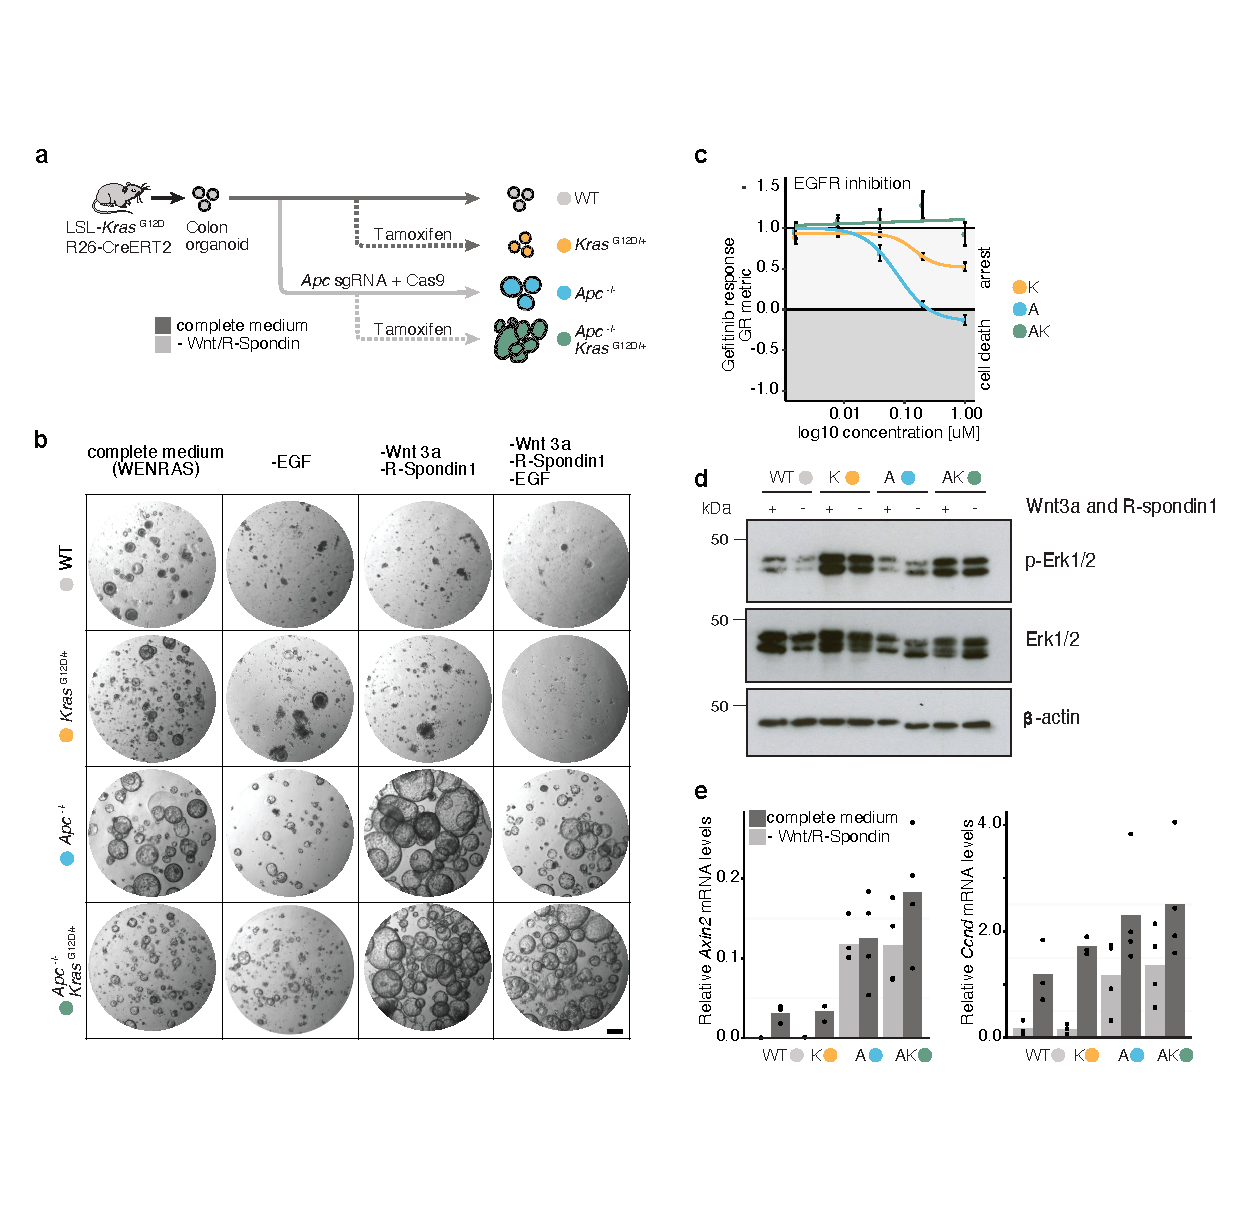
\includegraphics[width=\textwidth,
                height=\textheight,
                keepaspectratio]{figures/adenomaprofiling/pdf/fig_1_0.pdf}
\caption[Establishing organoid models of colon adenoma]{\textbf{Establishing organoid models of colon adenoma, a} Overview of organoid model establishment. Mouse colon organoids were isolated from a transgenic donor animal carrying an inactive conditional oncogenic \textit{Kras}\textsuperscript{G12D} allele. Homozygous truncation of \textit{Apc} via CRISPR and activation of the heterozygous \textit{Kras}\textsuperscript{G12D} allele lead to four different genetically defined organoid models.
\textbf{b} In vitro growth factor dependency of adenoma models. Organoids were cultured in complete or modified medium containing combinations of Wnt3A, R-Spondin1-Fc and Egf for 120h and subsequently imaged. Scalebar = 200µm.
\textbf{c}	Oncogenic \textit{Kras}\textsuperscript{G12D} increases resistance to Egfr inhibition. Organoid ATP levels were measured 4 days after Gefitinib treatment and adjusted for organoid growth rate. Points represent mean of n=2 independent experiments. Error bars represent standard error of mean.
\textbf{d} Erk phosphorylation is increased by oncogenic \textit{Kras}\textsuperscript{G12D}. Organoid models were cultured with or without Wnt3A and R-Spondin1-Fc for 72h and analyzed for protein levels. p, phospho.   
\textbf{e}	Loss of \textit{Apc} induces transcription of canonical Wnt-signaling target genes. qRT–PCR for Axin2 and Ccnd in the presence or absence of Wnt 3a and R-spondin1-Fc after 120h of culture. Expression levels are normalized to Sdha and Hprt transcript abundance. Bar graphs represent the mean of n=4 independent experiments. Wilcoxon rank sum test 
}
\label{fig_a10}
\end{figure}
\bigbreak

To model the formation of colon adenomas in vitro, I used a transgenic mouse to derive organoid cultures. The transgenic animal carried a conditional tamoxifen inducible \textit{Kras}\textsuperscript{G12D/+} allele \citep{jacksonAnalysisLungTumor2001} (Figure \ref{fig_a10} a). After isolation, I confirmed that extracted colon organoids did not express an activated form of \textit{Kras}\textsuperscript{G12D} (Figure \ref{fig_a11}a) and defined these organoids as wildtype (WT). To model loss-of-function mutations of the tumor suppressor \textit{Apc}, the ortholog of the frequently mutated mutation-cluster-region on the \textit{Apc} gene was targeted by CRISPR (Figure \ref{fig_a10} a). Generated organoids harbored biallelic loss-of-function mutations in \textit{Apc} (Figure \ref{fig_a11}a). Subsequent activation of oncogenic \textit{Kras}\textsuperscript{G12D/+} by treatment with 4-Hydroxytamoxifen led to four distinct organoid adenoma models (Figure \ref{fig_a10} a and Figure \ref{fig_a11}a-b); wildtype (WT), \textit{Apc}\textsuperscript{-/-}
  (A), \textit{Kras}\textsuperscript{G12D/+} (K), and \textit{Apc}\textsuperscript{-/-} / \textit{Kras}\textsuperscript{G12D/+} (AK).


\begin{figure}[h]
\centering
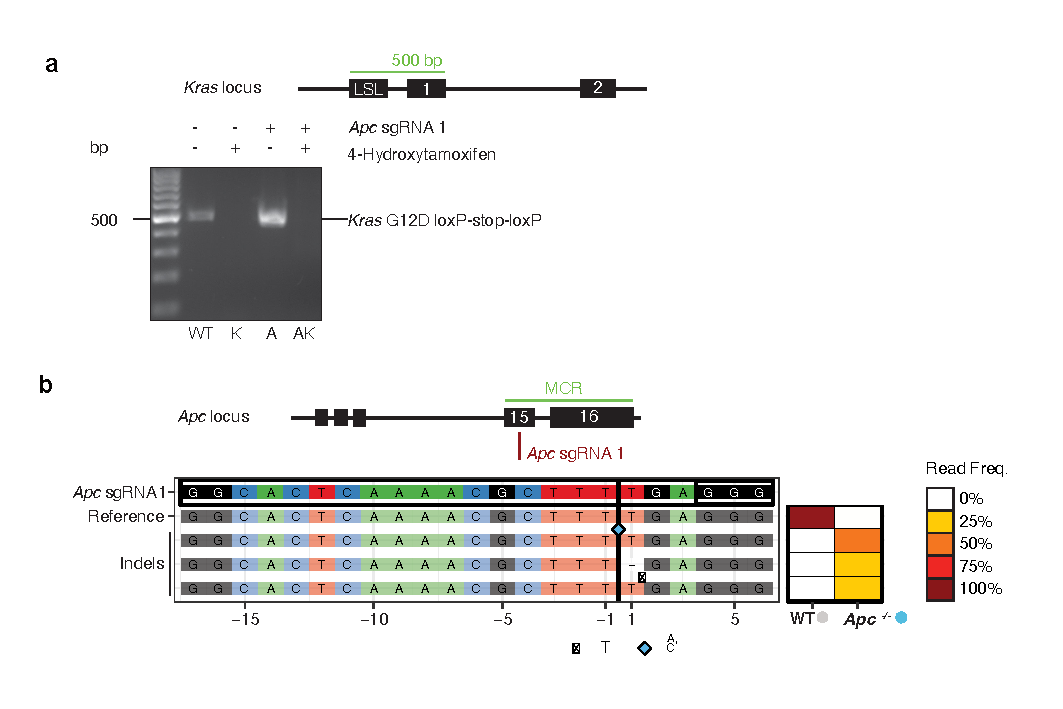
\includegraphics[width=\textwidth,
                height=\textheight,
                keepaspectratio]{figures/adenomaprofiling/pdf/fig_1_1.pdf}
\caption[Structural validation of organoid colon adenoma models]{\textbf{Structural validation of organoid colon adenoma models, a} Allele-specific PCR products of colon organoid models isolated from a transgenic mouse with a conditional tamoxifen inducible \textit{Kras}\textsuperscript{G12D/+} allele.
\textbf{b} Amplicon sequencing result of the murine mutation cluster region ortholog for organoids transfected with an \textit{Apc} targeting sgRNA and Cas9 carrying plasmid. The sequencing results show the presence of 3 different insertion/deletions within the pool of sgRNA treated organoid models. Wildtype sequences are absent within the CRISPR targeted pool, while mutant sequences are absent in the untreated organoid pool.}
\label{fig_a11}
\end{figure}
\bigbreak

Similar to genetically modified human colon organoids \citep{drostSequentialCancerMutations2015, matanoModelingColorectalCancer2015a}, murine colon organoids showed characteristic niche requirements. Both \textit{Apc} mutant organoid lines grew independent of the Wnt-signaling activating factors Wnt 3a and R-Spondin1 (Figure \ref{fig_a10} b) and at an accelerated proliferation rate. In fact, \textit{Apc} mutant lines showed an increased growth in a Wnt3a and R-Spondin1 free environment when compared to the complete medium. Organoid models with an activated \textit{Kras}\textsuperscript{G12D} allele were less sensitive to removal of EGF from the media. However, as observed before \citep{drostSequentialCancerMutations2015}, the mutant \textit{Kras}\textsuperscript{G12D} allele was insufficient to compensate completely for the loss of EGF from the medium. Nevertheless, \textit{Kras}\textsuperscript{G12D} mutant organoid lines were more resistant to pharmacological inhibition of Egfr signaling (Figure \ref{fig_a10} c). In conclusion, organoid model genotypes were reflected in characteristic growth factor dependencies in experimental conditions.

\bigbreak
Next, I investigated the effects of mutations in \textit{Apc} and \textit{Kras} on both canonical Wnt- and Erk dependent signaling. While the presence of the \textit{Kras}\textsuperscript{G12D/+} allele led to an increase in Erk-phosphorylation across models, \textit{Apc}\textsuperscript{-/-} / \textit{Kras}\textsuperscript{G12D/+} organoids showed no marked additional increase in Erk-phosphorylation when compared to \textit{Kras}\textsuperscript{G12D/+} organoids (Figure \ref{fig_a10} d). Moreover, \textit{Apc}\textsuperscript{-/-} / \textit{Kras}\textsuperscript{G12D/+} adenoma models showed no significant differences in expression of the Wnt target genes \textit{Axin2} and \textit{Ccnd} when compared to \textit{Apc}\textsuperscript{-/-}  single-mutant models (A) (p > 0.34 for all conditions, Wilcoxon rank sum test) (Figure \ref{fig_a10} e). These results indicate that organoid adenoma models show genotype-dependent activity of characteristic signaling pathways, while there is no extensive crosstalk between the \textit{Apc}\textsuperscript{-/-}   and \textit{Kras}\textsuperscript{G12D/+} allele in mouse colon organoids that that is directly reflected in canonical Wnt- and Erk dependent signaling.  

\bigbreak
\subsection{Molecular characterisation of organoid models}
To comprehensively characterise the four organoid models, transcriptome, proteome and lipidome profiling were performed using mRNA microarrays and mass spectrometry, respectively (Figure \ref{fig_161}). For these measurements organoids were kept in the same culture condition and duration that were used during the subsequent image-based profiling experiment: After passaging, all organoids were kept in Wnt 3a, R-Spondin1 rich medium (WENRAS) to model conditions within the niche and stimulate outgrowth before the medium was changed to a Wnt 3a-free medium (ENR) to model conditions outside the niche. The medium was supplemented with EGF both before and after the medium change. Transcriptome profiling of organoid models showed an increased expression of the stem-cell marker Lgr5 and negative Wnt-signaling regulators such as \textit{Nkd1}, \textit{Notum}, \textit{Wif1} and \textit{Znrf3} in \textit{Apc} mutant organoid lines (Figure \ref{fig_160} b). In contrast, \textit{Apc} wildtype organoid lines showed an increased expression of epithelial differentiation markers, such as \textit{Krt20}, \textit{Alpp} and \textit{Abcb1} (P-glycoprotein). Overall, the number of genes with significant expression changes after \textit{Apc} loss was 2.5 times greater compared to isolated \textit{Kras}\textsuperscript{G12D} activation (FDR = 0.1, \textit{Apc}\textsuperscript{-/-} : 44.5\%, \textit{Kras}\textsuperscript{G12D/+}: 18.3\% of assessed genes). A related observation was made during the analysis of protein abundance. Again, Wnt signaling regulators (Axin2, Notum) were enriched in \textit{Apc} mutant organoid lines and the number of significantly regulated proteins after \textit{Apc} loss was 2.5 times greater compared to an isolated \textit{Kras}\textsuperscript{G12D} activation (FDR = 0.1, \textit{Apc}\textsuperscript{-/-} : 260, \textit{Kras}\textsuperscript{G12D/+}: 105 assessed proteins). Principal component analysis of both transcriptome, proteome and lipidome data showed related axes of variation across measurements. In all observed modalities, the first principal component captured differences between \textit{Apc} wildtype and \textit{Apc} mutant organoid models, while the second (in case of proteomics measurements the third) principal component captured differences between wildtype and \textit{Kras}\textsuperscript{G12D/+} single-mutant models (Figure \ref{fig_161}b, \ref{fig_161}c and \ref{fig_161}d). In every modality, a high degree of similarity was observed among \textit{Apc}\textsuperscript{-/-}  and \textit{Apc}\textsuperscript{-/-} / \textit{Kras}\textsuperscript{G12D/+} organoid lines. While activation of oncogenic \textit{Kras}\textsuperscript{G12D} in wildtype organoids led to global changes in transcript, protein and lipid expression, these changes were not as pronounced in organoids without functional \textit{Apc}. In fact, only the mRNA expression of 91 genes was significantly altered between \textit{Apc}\textsuperscript{-/-}  and \textit{Apc}\textsuperscript{-/-} / \textit{Kras}\textsuperscript{G12D/+} organoids (FDR = 0.1). 

\begin{figure}[H]
\centering
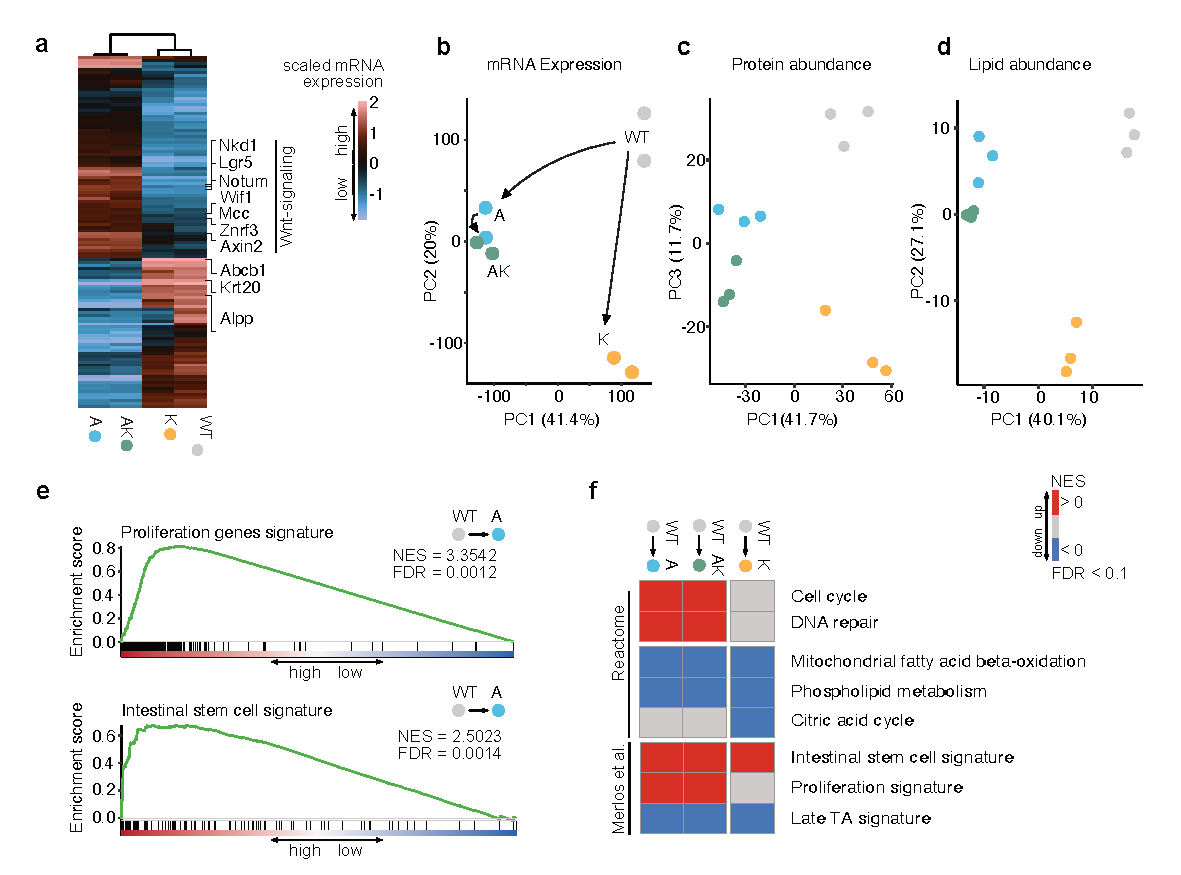
\includegraphics[width=\textwidth,
                height=\textheight,
                keepaspectratio]{figures/adenomaprofiling/pdf/fig_1_6_1_2.pdf}
\caption[Molecular characterisation of organoid adenoma models]{\textbf{Molecular characterisation of organoid adenoma models. a} Differential gene expression of adenoma models. Shown are scaled expression values for the top 125 differentially expressed genes for every organoid line. Selected genes are highlighted. All organoids were cultured for 3 days in WENRAS before exposure to ENR for 4 days. Cell number was controlled between experiments. Whole organoid lysates were analyzed. 
\textbf{b} Transcript abundance data. Shown are the first two principal components of scaled gene expression data. The proportion of variance of each principal component is listed in parenthesis. 
\textbf{c} Protein abundance data. Shown are the first and third principal component of scaled protein expression data. The proportion of variance of each principal component is listed in parenthesis. 
\textbf{d} Lipid species abundance data. Shown are the first two principal components of scaled lipid abundance data. The proportion of variance of each principal component is listed in parenthesis. 
\textbf{e} Loss of \textit{Apc} leads to increased expression of proliferation and intestinal stem cell associated genes. Shown is a gene set enrichment analysis of differentially expressed genes between \textit{Apc} mutant and WT organoids. Intestinal gene expression signatures were used according to Merlos-Suarez et al. NES, normalized enrichment score. 
\textbf{f} Overview of cellular processes in organoid adenoma models. Shown are selected enriched differential gene expression signatures from Reactome and Merlos-Suarez et al. NES, normalized enrichment score. NES > 0 suggests an enriched/ activated biological process. FDR < 0.1.}
\label{fig_161}
\end{figure}
\bigbreak

To explore active biological processes, gene set enrichment analysis on organoid transcript expression data was performed. The strongest changes in expression after loss of \textit{Apc} were linked to an increased proliferation rate (Figure \ref{fig_160} e). Gene set enrichment analysis of published intestinal cell-proliferation and stem cell signatures showed an enrichment of both signatures in \textit{Apc}\textsuperscript{-/-}  organoids (Figure \ref{fig_160} e) \citep{merlos-suarezIntestinalStemCell2011}. In contrast, a signature for differentiating, transit-amplifying cells was depleted. Gene set enrichment analysis of \textit{Apc}\textsuperscript{-/-} / \textit{Kras}\textsuperscript{G12D/+} double-mutant organoids showed the same results. Next to these published signatures, I explored the enrichment of curated gene sets from the Reactome database \citep{grissReactomeGSAEfficientMultiOmics2020}. Here, both \textit{Apc}\textsuperscript{-/-}  and \textit{Apc}\textsuperscript{-/-} / \textit{Kras}\textsuperscript{G12D/+} double-mutant lines showed a positive enrichment of cell cycle and DNA repair related genes when compared to wildtype organoids (Figure \ref{fig_162}a). Unique to the \textit{Kras}\textsuperscript{G12D/+} organoid line was a decreased expression of citric acid cycle and respiratory chain related genes (Figure \ref{fig_162}b). This effect, was not observed in \textit{Apc}\textsuperscript{-/-} / \textit{Kras}\textsuperscript{G12D/+} double mutant organoids (Figure \ref{fig_161}f). In addition, organoid models with an \textit{Kras}\textsuperscript{G12D/+} genotype showed a downregulation of the \textit{Egfr} receptor, in line with a potential negative feedback response to hyperactivated ERK-MAPK signaling (Figure \ref{fig_162}b). Both \textit{Apc}\textsuperscript{-/-}  and \textit{Kras}\textsuperscript{G12D/+} organoid models showed a strong reduction of lipid metabolism and beta-oxidation (Figure \ref{fig_162}a,b). In summary, (1) loss of \textit{Apc} leads to a global shift in transcript, protein, and lipid composition in colon organoids, including a strong increase in cell proliferation associated transcripts; (2) Activation of isolated oncogenic \textit{Kras}\textsuperscript{G12D} leads to pronounced reduction in citric acid cycle related transcripts while this phenotype was not seen in organoid models with an additional loss of \textit{Apc}; (3) Both \textit{Apc} loss and activation of oncogenic \textit{Kras}\textsuperscript{G12D} lead to a reduction of lipid beta-oxidation related transcripts.

\begin{figure}[h]
\centering
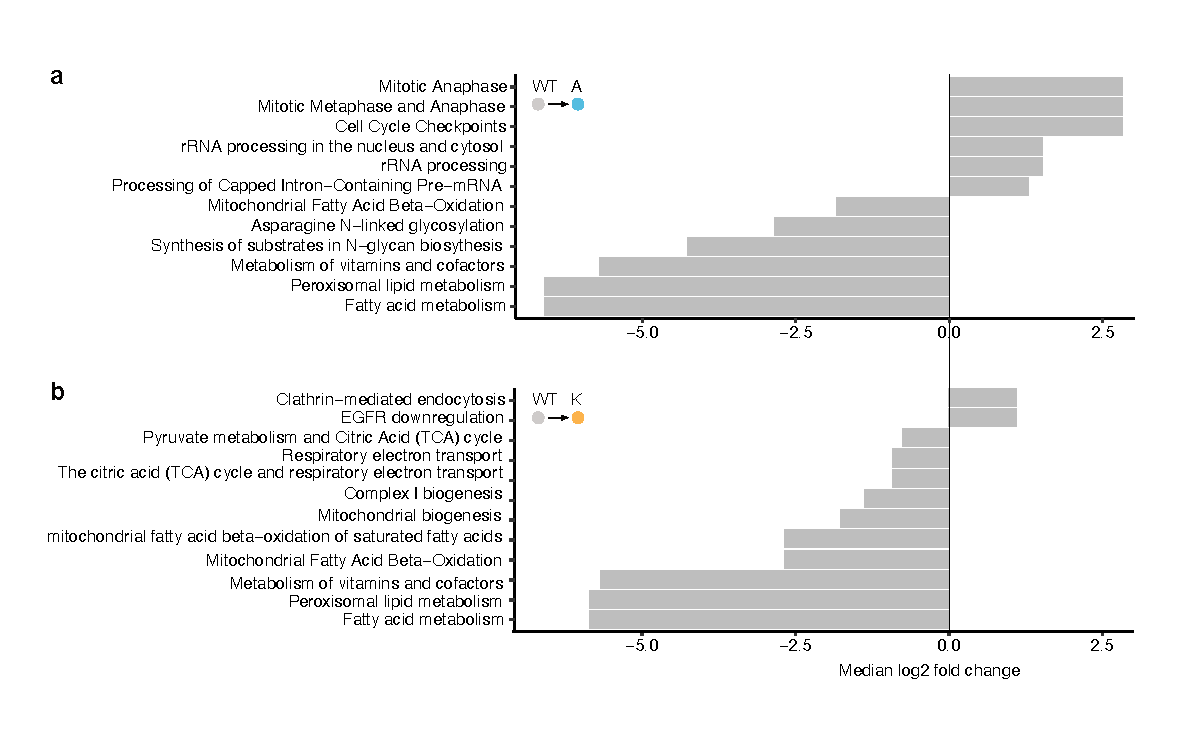
\includegraphics[width=\textwidth,
                height=\textheight,
                keepaspectratio]{figures/adenomaprofiling/pdf/fig_1_6_2.pdf}
\caption[Representative up and down-regulated transcriptional processes after loss of \textit{Apc} and activation of oncogenic \textit{Kras}\textsuperscript{G12D}]{
\textbf{a} Representative up and down-regulated transcriptional processes after loss of \textit{Apc}. Expression signatures were sourced from Reactome and average log2 fold changes for included transcripts are illustrated. FDR < 0.1.
\textbf{b} Representative up and down-regulated transcriptional processes after activation of oncogenic \textit{Kras}\textsuperscript{G12D}. Expression signatures were sourced from Reactome and average log2 fold changes for included transcripts are shown. FDR < 0.1.
}
\label{fig_162}
\end{figure}
\bigbreak

To further understand the pronounced changes in fatty acid metabolism observed in both \textit{Apc}\textsuperscript{-/-}  and \textit{Kras}\textsuperscript{G12D/+} organoid models, differences in lipid composition were measured using untargeted lipid extraction and Mass Spectrometry. In total, more than 350 lipids from 15 species were identified across all samples (Figure \ref{fig_168} a). The majority of identified lipids had fatty acid chain lengths of 20 to 40 carbon atoms, while Triglycerides (TAG) had an increased length of 40 to 60 carbon atoms (Figure \ref{fig_168} b). Major differences between organoid lines were seen especially for storage lipids - Triglycerides (TAG) and Cholesterol Esters (CE) (Figure \ref{fig_168} c and d, respectively). Both lipid species were more abundant in the two \textit{Apc}\textsuperscript{-/-}  organoid lines (p < 0.05, TAG: t > 4.8, CE: t > 3.7, ANOVA). In single-mutant \textit{Kras}\textsuperscript{G12D/+} organoids, Triglycerides were also more abundant compared to wildtype organoids (p < 0.05, t = 5.9, ANOVA), while Cholesterol esters were depleted (p < 0.05, t = -3.7, ANOVA). The increase in the abundance of storage lipids as a result of \textit{Apc} loss of function and oncogenic \textit{Kras}\textsuperscript{G12D} mutation were aligned with the transcriptional changes that indicated a reduced rate of beta-oxidation in these models (Figure \ref{fig_162}a,b). 

\begin{figure}[h]
\centering
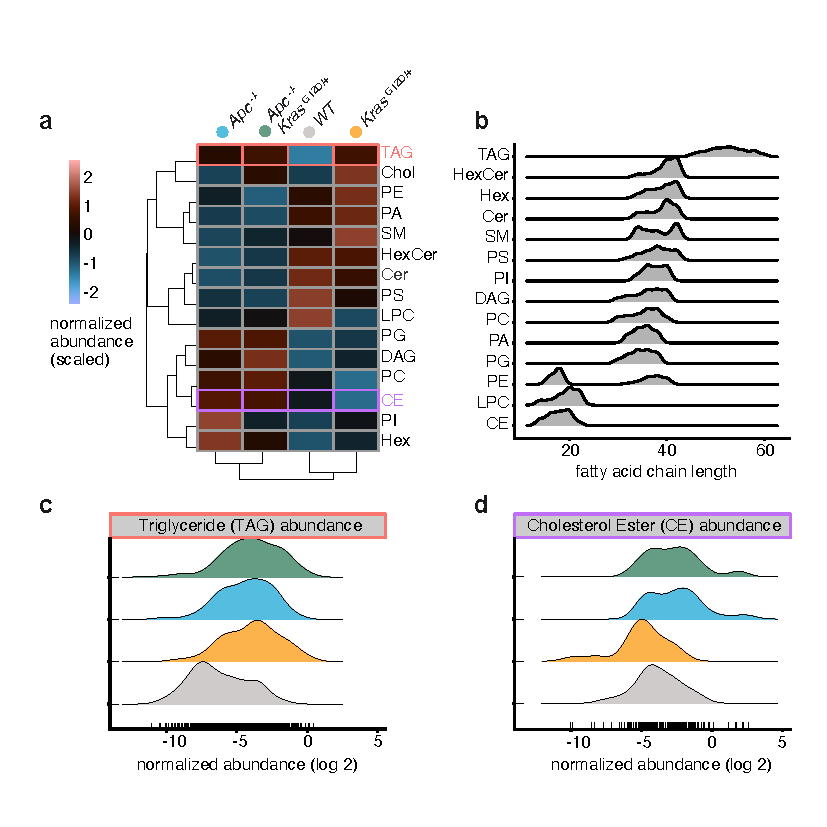
\includegraphics[width=350,
                height=\textheight,
                keepaspectratio]{figures/adenomaprofiling/pdf/fig_1_6_8.pdf}
\caption[Lipid composition changes across organoid adenoma models]{\textbf{Lipid composition changes across organoid adenoma models. a} Lipid species abundance of adenoma models. Shown are scaled abundance values for major lipid species for every organoid line. Selected lipid species are highlighted (Lipid Maps Abbreviations: HexCer - Hexosylceramide; PA - Phosphatidate; Cer - Ceramide; SM - Sphingomyelin; LPC - Lysophosphatidylcholine; PS - Phosphatidylserine; PE - Phosphatidylethanolamine; PI - Phosphatidylinositol; PG - Phosphatidylglycerol; DAG - Diacylglycerol; PC - Phosphatidylcholine; TAG - Triacylglycerol; Hex2Cer - Dihexosylceramide; CE - Cholersterolester, Chol - Cholesterol). All organoids were cultured for 3 days in WENRAS before exposure to ENR for 4 days. Cell number was controlled between experiments. Whole organoid lysates were analyzed. 
\textbf{b} Fatty acid chain lengths by lipid species. Shown are the distribution of fatty acid chain lengths.
\textbf{c} Distribution of Triacylglycerol (TAG) abundance across organoid adenoma models. ANOVA was performed to model average lipid abundance as a function of organoid line across replicates.
\textbf{d} Distribution of Cholesterolester (CE) abundance across organoid adenoma models. ANOVA was performed to model average lipid abundance as a function of organoid line across replicates.
}
\label{fig_168}
\end{figure}
\bigbreak


\newpage
\section{Image-based profiling of organoid models}

\begin{figure}[h!]
\centering
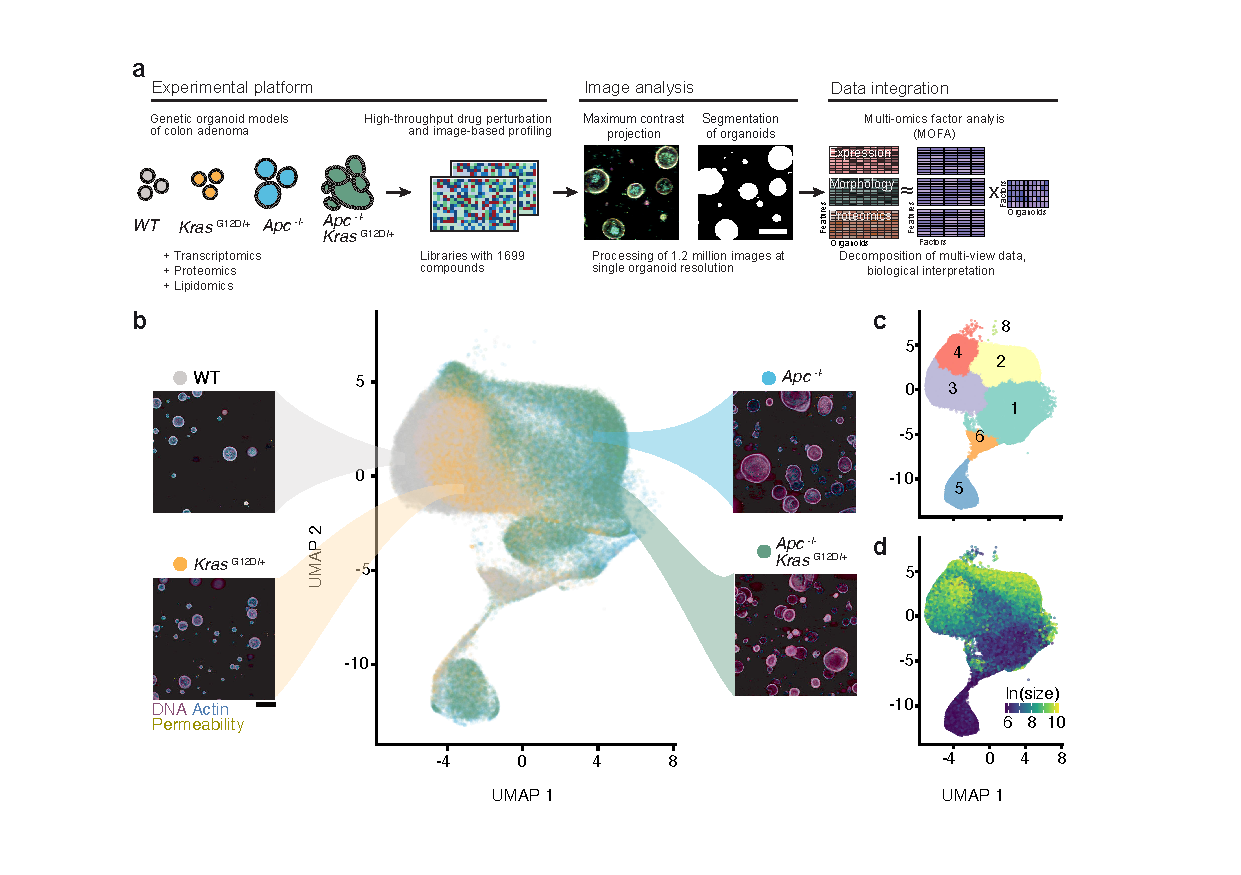
\includegraphics[width=\textwidth,
                height=\textheight,
                keepaspectratio]{figures/adenomaprofiling/pdf/fig_1_2.pdf}
\caption[Image-based profiling of organoid adenoma models]{\textbf{Image-based profiling of organoid adenoma models. a} Overview of experiments. Organoids were isolated from a transgenic mouse model and genetically edited. Organoids were dissociated and evenly seeded in 384-well plates before perturbation with an experimental small molecule library. After treatment, high-throughput fluorescence microscopy was used to capture the morphology of organoids in 16 selected z-layers and 3 channels. 3D imaging data were projected on a 2D plane using a maximum contrast projection. Here, only pixel areas with the largest contrast among the z-axis were retained. Morphological features were computed based on the projection. Untreated organoid morphology, organoid size and treatment activity scores were integrated with transcript expression, protein abundance, lipid abundance and genogtype data in a Multi-Omics Factor Analysis (MOFA) model. Figure created with support from Johannes Betge (graphical presentation). 
\textbf{b} Uniform Manifold Approximation and Projection (UMAP) of organoid-level features for a random 5\% sample out of imaged organoids. The identical sample is used for visualizations throughout the figure. Organoid genotype is colorcoded and representative images are displayed (magenta = DNA, cyan = actin, cell permeability = yellow, scale-bar: 200µm). \textbf{c} Graph-based clustering of organoids by morphology with 8 resulting clusters. \textbf{d} Organoid size distribution. Color corresponds to the log-scaled organoid area (dark blue: minimum size, yellow: maximum size).}
\label{fig_120}
\end{figure}
\bigbreak

\subsection{Single-Organoid level phenotypes are organised by model genotypes}
Once models were characterised on a molecular level, the previously developed image-based profiling approach was applied. Organoid models of the four different genotypes were perturbed with a library of ca. 1700 compounds and morphological profiles were systematically observed (Figure \ref{fig_120} a). As previously described, classic morphological features were collected for single organoids, normalised, and principal components were calculated, of which 25 components (accounting for >80\% of the variance) were retained and used throughout the further analysis. A UMAP projection of single-organoid morphology showed distinct genotype-dependent morphological states for identified organoids (Figure \ref{fig_120} b). Graph based clustering of organoid morphology profiles resulted in 8 clusters (Figure \ref{fig_120} c). Organoids within cluster 4 and 3 were enriched for \textit{Apc}\textsuperscript{+/+} organoid models, cluster 2 and 1 were populated by \textit{Apc}\textsuperscript{-/-}  models. Analogous to gene expression, lipidomics and proteomics representation space, the two \textit{Apc} mutant organoid models were less distinct from each other than organoids with a WT and isolated \textit{Kras}\textsuperscript{G12D/+} genotype (Figure \ref{fig_140} b). While developed organoids that present with a larger organoid area showed distinct genotype-specific morphologies, small organoids and non-viable organoid fragments clustered together across genotypes within cluster 5 (Figure \ref{fig_120} c and d). The distribution of DMSO-treated organoids and small molecule perturbed organoids in morphological space overlapped considerably (Figure \ref{fig_140} a), most likely because many treatments were inactive and did not alter organoid morphology. 

\bigbreak
\begin{figure}[h!]
\centering
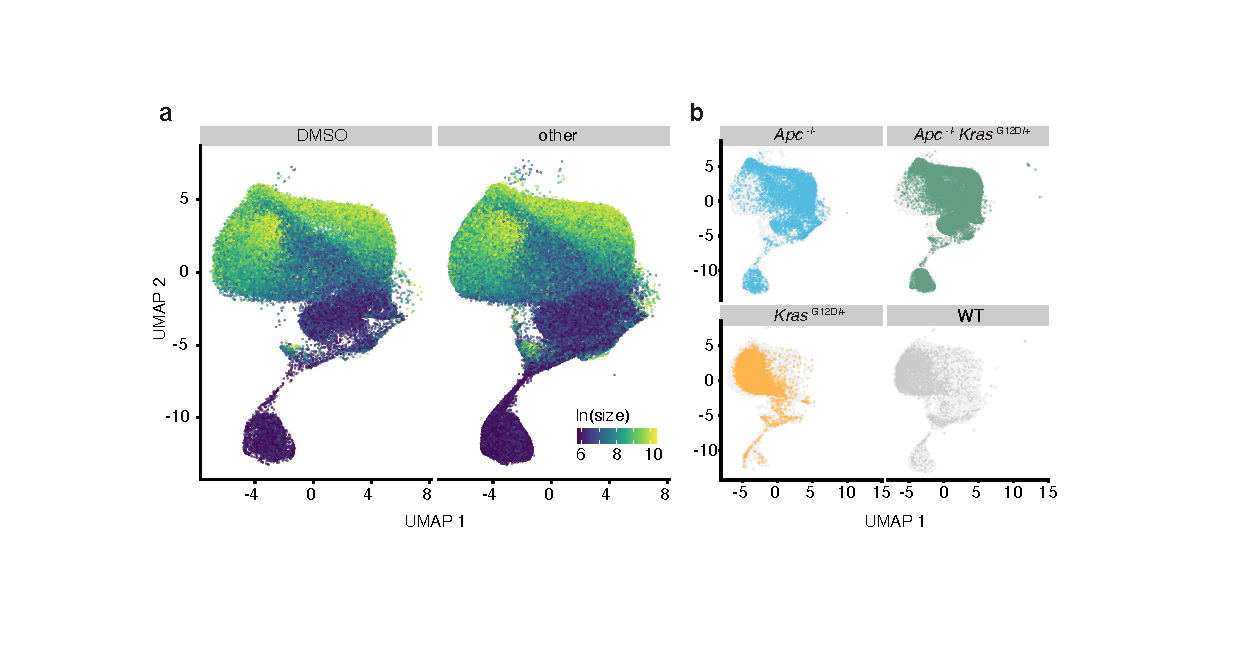
\includegraphics[width=\textwidth,
                height=\textheight,
                keepaspectratio]{figures/adenomaprofiling/pdf/fig_1_4.pdf}
\caption[Treatment and genotype dependent effects within the organoid morphology distribution]{\textbf{Treatment and genotype dependent effects within the organoid morphology distribution. a} UMAP representation of DMSO treated (vehicle) and small molecule treated organoids. \textbf{b}, UMAP embeddings of four organoid genotypes (baseline state = 0.1\% DMSO control-treated organoids), grey background consists of randomly sampled organoids.}
\label{fig_140}
\end{figure}

When comparing the morphologies of different organoid lines in detail, characteristic differences were identifiable (Figure \ref{fig_130} a). DMSO-treated \textit{Apc}\textsuperscript{+/+} organoids showed a strong, regular apical actin cytoskeleton (high average actin intensity) that organized the multicellular formation into a regular-patterned spherical morphology (low average eccentricity). In contrast, \textit{Apc}\textsuperscript{-/-}  organoids showed a relative lack of a regular actin cytoskeleton (low average actin intensity) and a irregular, non-spherical morphology (high average eccentricity). In summary, organoid models showed genotype-dependent differences in morphology. Analogous to differences in molecular state, a primary source of variation was caused by loss of the tumor suppressor gene \textit{Apc}. Organoids with truncated \textit{Apc} presented with a higher proliferation rate, increased overall DNA staining intensity and loss of the regular spherical apical actin cytoskeleton that was observed in \textit{Apc}\textsuperscript{+/+} organoid models.

\begin{figure}[h!]
\centering
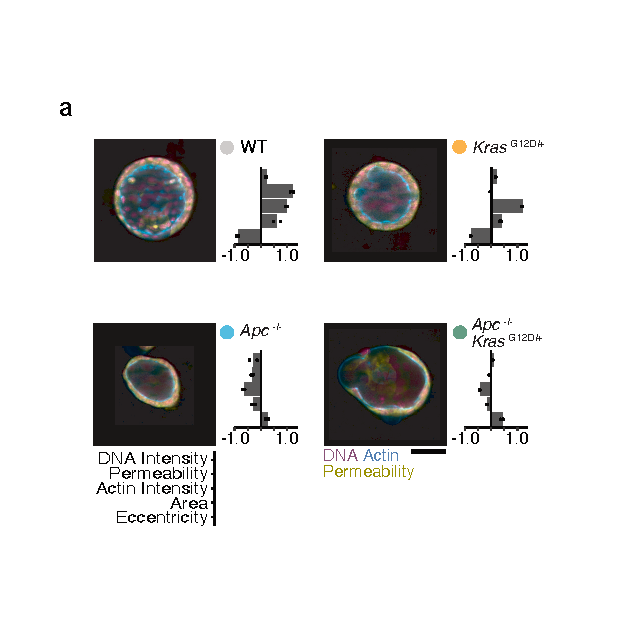
\includegraphics[width=200,
                height=\textheight,
                keepaspectratio]{figures/adenomaprofiling/pdf/fig_1_3.pdf}
\caption[Genotype dependent effects on organoid morphology]{\textbf{Genotype dependent effects on organoid morphology. a}  Morphological organoid profiles from vehicle-treated adenoma models were aggregated. Shown are representative individual organoids with selected features. Points show the mean phenotype for each independent biological replicate. Representative, interpretable features and their z-scores relative to all single organoid profiles are shown (magenta = DNA, cyan = actin, cell permeability = yellow, scale-bar: 25µm)}
\label{fig_130}
\end{figure}
\bigbreak



\subsection{Scoring small molecule induced phenotypes across organoid models}

\begin{figure}[h!]
\centering
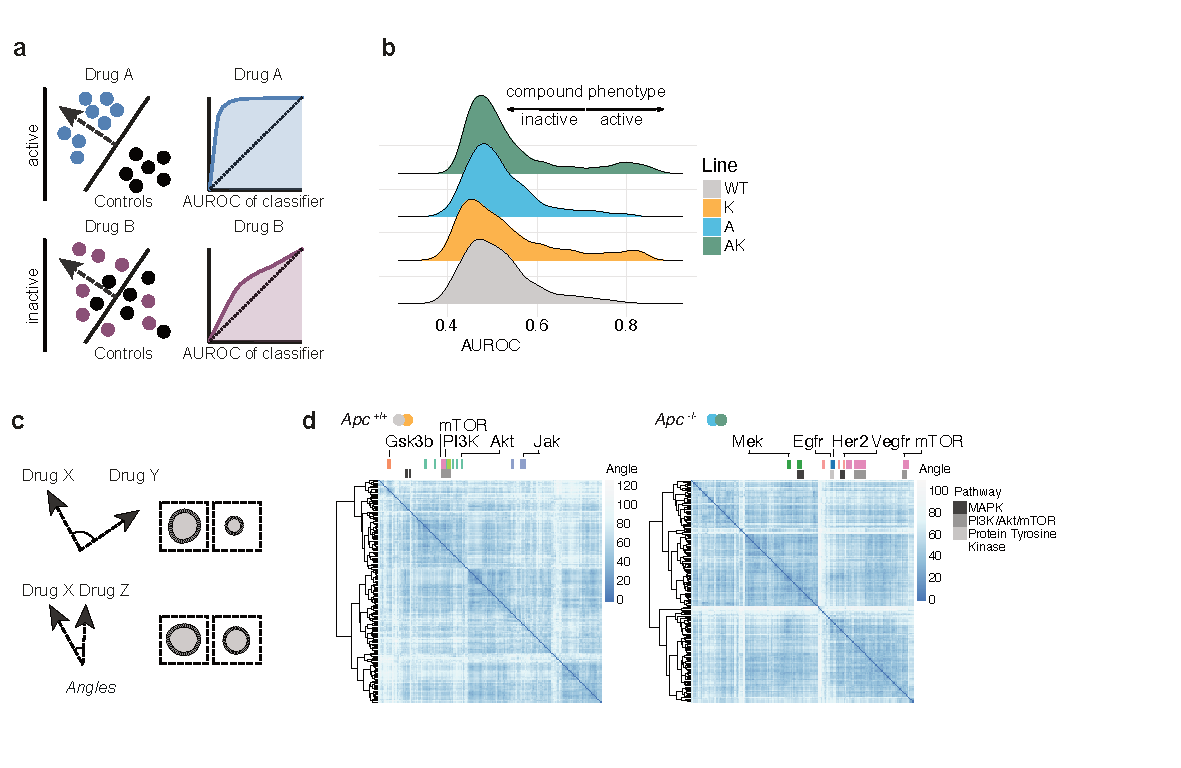
\includegraphics[width=\textwidth,
                height=\textheight,
                keepaspectratio]{figures/adenomaprofiling/pdf/fig_1_5_2.pdf}
\caption[Treatment activity scoring]{\textbf{Treatment activity scoring. a} A logistic regression classifier is trained to distinguish morphology profiles of individual treated and untreated organoids across all available replicates. Afterwards, the classifier is applied to a validation set of organoids and the classification performance is estimated using the area under the receiver operating characteristic curve (AUROC) metric. Method implemented by Jan Sauer.
\textbf{b} Distribution of treatment activity scores for all organoid lines, replicates and perturbations. 
\textbf{c} Identifying related treatment induced phenotypes. Normal vectors of treatment specific classifiers were compared by calculating the angular distance (related to cosine similarity, ranging from 0-180 degrees). Small angular distance between vectors correspond to a high similarity between the treatment-induced organoid phenotypes. Method implemented by Jan Sauer.
\textbf{d} A clustered heatmap of compound induced phenotypes for \textit{Apc} mutant and \textit{Apc} wildtype organoids. Highlighted are clusters of compound induced phenotypes with related targets. Normal vectors for \textit{Apc} mutant and \textit{Apc} wildtype organoids were concatenated before angular distance calculation. Method implemented by Jan Sauer.
}
\label{fig_150}
\end{figure}
\bigbreak

After identifying genotype-dependent morphological differences, the next step was to explore effects of small molecule treatment on different organoid models. To describe the activity of a treatment, the classification-based approach developed during the study of human cancer organoid phenotypes in the previous chapter was used. Briefly, for every treatment and genotype, a logistic regression classifier was trained to distinguish DMSO-treated organoids from treated organoids. The classification performance, expressed as the AUROC, was used to determine the activity of a treatment. A high AUROC score (approaching 1) is observed for compounds that lead to a treatment-induced organoid morphology that is very distinct from DMSO treated organoids. In contrast a low AUROC (centered around 0.5) is observed for compounds where the model's classification performance approaches random guessing (Figure \ref{fig_150} a). The distribution of activity scores across organoid lines showed that most compounds did not lead to an identifyable morphological change (Figure \ref{fig_150} b) and showed AUROC values centered around 0.5. Next to identifying differences around the number of active treatments, I was interested what small molecules were active in a given organoid genotype and their treatment-induced morphology change. Based on the observation that the primary source of variation for treatment activity was the state of the \textit{Apc} allele, organoid lines were aggregated by their \textit{Apc} allele for further analysis. In line with the approach taken in the previous chapter, normal vectors of the logistic regression classifiers were compared using the cosine distance (Figure \ref{fig_150} d). The resulting clustering of treatments showed an enrichment for small molecules with related mechanism of action (Figure \ref{fig_150} e and f). For example, Egfr inhibitors were significantly enriched in \textit{Apc}-mutant organoid lines, while GSK3B-inhibitors, which lead to a stimulation of canonical Wnt signaling, were only enriched in \textit{Apc}-wildtype organoid models. To summarise the findings above, organoid models showed genotype-specific treatment-induced phenotypes. For example, GSK3B-inhibitors were active in \textit{Apc}\textsuperscript{+/+} organoids and showed a characteristic treatment-induced phenotype in these models.

\section{Multi-omics factor analysis identifies shared factors linking functional and structural biological views}

\subsection{Learning a multi-view representation with MOFA}

\begin{figure}[h!]
\centering
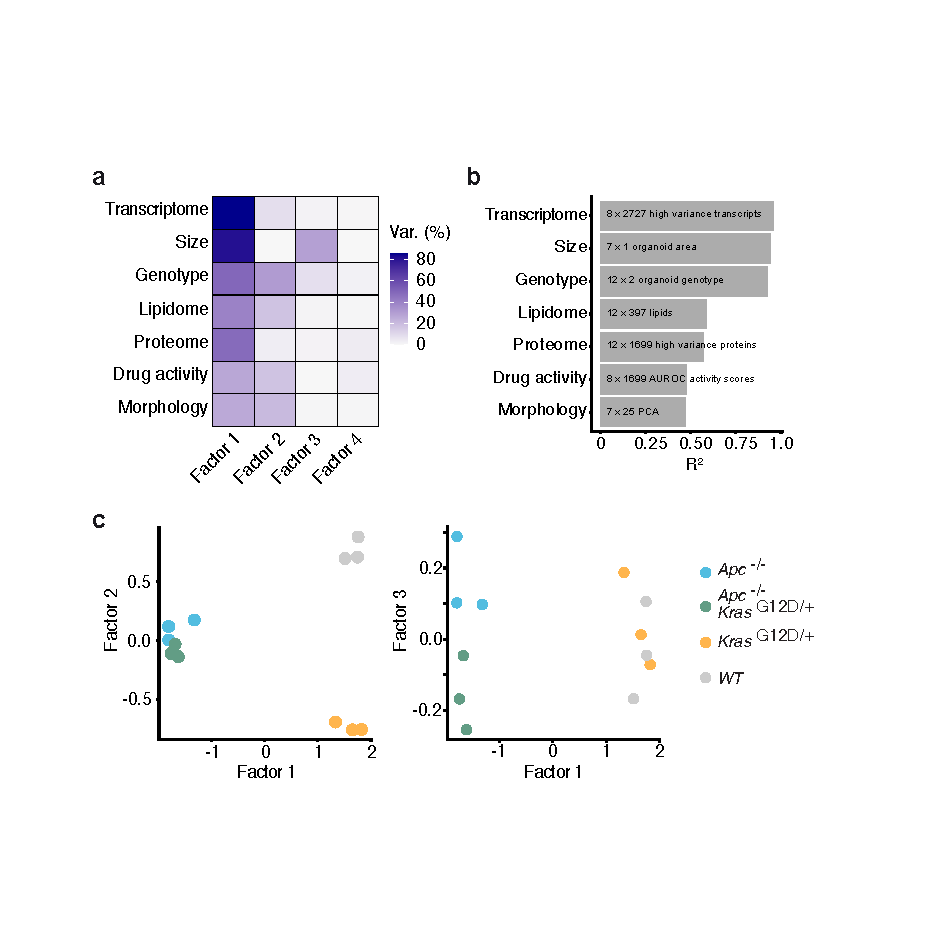
\includegraphics[width=400,
                height=\textheight,
                keepaspectratio]{figures/adenomaprofiling/pdf/fig_1_7.pdf}
\caption[Multi-omics factor analysis (MOFA) to identify shared factors linking morphology, size, gene expression, lipidomics, proteomics, genotype and treatment activity]{\textbf{Multi-omics factor analysis (MOFA) to identify shared factors linking morphology, size, gene expression, lipidomics, proteomics, genotype and treatment activity. a} Percent variance explained by the MOFA model for each factor. Untreated organoid morphology, organoid size and treatment activity scores were integrated with genotype, proteomics, lipidomics and mRNA expression data. \textbf{b} Cumulative proportion of total variance explained by each experimental data modality within the MOFA model. \textbf{c}, Visualization of samples in factor space showing factors 1 and 2 as well as factor 1 and 3. Shown are independent replicates for each organoid line. 
}
\label{fig_170}
\end{figure}
\bigbreak

To jointly model the biological and morphological state of the four organoid lines, I performed multi-omics factor analysis (MOFA). Analogous to the process described in the previous chapter, molecular and morphological features from untreated organoids were factorized using k=4 factors (Figure \ref{fig_170} a and \ref{fig_180} a). The learned model was based on both morphological (e.g. morphology, size, small molecule activity) and molecular (e.g. genotype, proteomics, lipidomics and transcript expression) information. To reduce the dimensionality of data modalities with a high number of features, only high variance features from gene expression and proteomics analysis were used. The resulting factorization explained the data ranging from ca. 90\% (gene expression) to 50\% (morphology) of explained variance (R\textsuperscript{2}) across the analyzed views. The first three factors captured the majority of variance, >40\%, ca. 10\%, and <10\%, respectively (Figure \ref{fig_170} a). The learned model explained most variance within the mRNA expression and genotype data, while measurements within the organoid morphology data had the lowest explained variance (Figure \ref{fig_170} b). When inspecting factor weights for the morphology domain, principal component 1, which accounted for ca. 30\% of variance within all observed (treated and untreated) morphology data during the image processing had small relative assigned feature weights across all learnt factors (from high to low absolute feature weight: rank 8/25, 11/25, 24/25 and 25/25 for factors 1 through 4, respectively). In contrast, principal components 2, 3, and 4 had the highest assigned feature weights across all four factors. In summary, MOFA was used to learn k=4 factors across a set of distinct data modalities. In the imaging domain, the learnt representation captured only a subspace of the observed morphological space, possibly because of high noise levels in morphological data and the fact that only observations from untreated organoids were contained in the modeled support set. 
\par

Visual inspection of factors as well as exploration of factor weights within the genotype view showed that factor 1 explained differences caused by \textit{Apc} loss of function, while factor 2 explained differences caused by the activation of \textit{Kras}\textsuperscript{G12D} in an \textit{Apc}\textsuperscript{+/+} genotype (Figure \ref{fig_170} c and \ref{fig_180} b). In contrast to factor 2, factor 3 captured differences between Kras+/+ and \textit{Kras}\textsuperscript{G12D/+} organoids with \textit{Apc} loss of function. While the number of factors is a user-defined hyperparameter within MOFA, the method automatically drops excess factors if they are not considered effective based on an applied automatic relevance determination (ARD) prior \citep{argelaguetMultiOmicsFactorAnalysis2018b}. Increasing the number of factors above k=4 in this analysis, did not lead to an increased number of interpretable factors. In fact, factor 4 already did not capture differences between organoid genoypes and was not interpretable from a biological point of view by the author (Figure \ref{fig_180} b). The determined number of explanatory factors corresponded to the hypothesized intrinsic dimensionality of the data: effects attributed to the \textit{Apc}\textsuperscript{-/-}  allele, the \textit{Kras}\textsuperscript{G12D} allele, and their interaction.

\begin{figure}[h!]
\centering
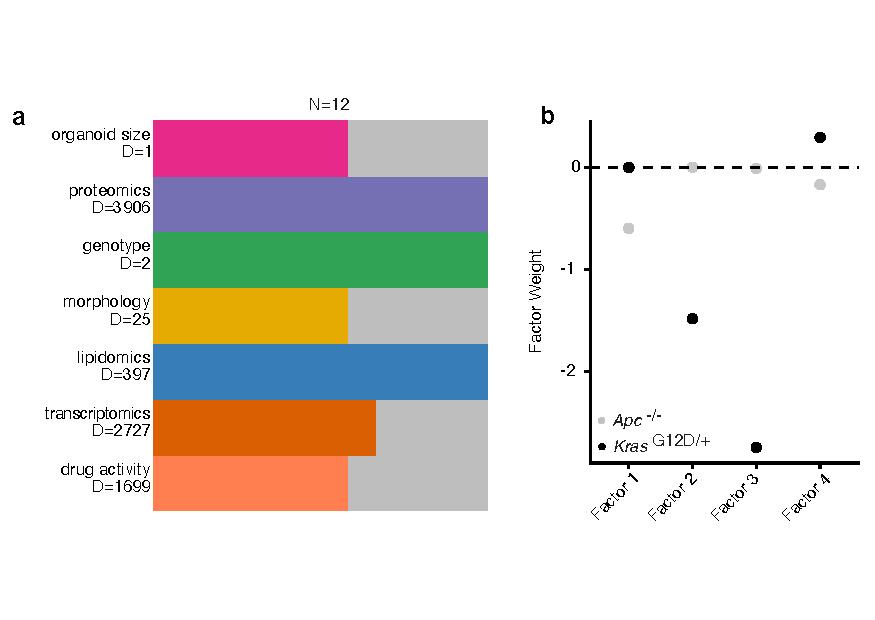
\includegraphics[width=400,
                height=\textheight,
                keepaspectratio]{figures/adenomaprofiling/pdf/fig_1_8.pdf}
\caption[Multi-omics factor analysis input data and loadings]{\textbf{Multi-omics factor analysis input data and loadings. a} measurement modalities, dimensionality and number of measurements. A third replicate of measurements were available for proteomics and lipidomics only. \textbf{b} Factor loadings for genotype information.} 
\label{fig_180}
\end{figure}
\bigbreak

\subsection{A canonical Wnt signaling associated program caused by \textit{Apc} loss}

To understand the molecular changes associated with factor 1, factor loadings for mRNA expression data were analyzed using Reactome gene-set enrichment analysis (Figure \ref{fig_190} a). Three clusters of biological processes were significantly associated with a negative factor loading, caused by \textit{Apc} loss-of-function: 1) Mitotic Anaphase related processes, including spindle checkpoints; 2) Mitotic S-phase, including DNA replication and 3) DNA repair mechanisms, including homology directed repair. In line with the enrichment of processes associated with cell proliferation, factor 1 loadings showed an enrichment of the previously described intestinal proliferation signature (Figure \ref{fig_190} c) and an LGR5+ instestinal stem cell identity signature (Figure \ref{fig_190} b). These findings are in line with the long-standing evidence that loss of \textit{Apc} leads to a hyperactivation of canonical Wnt signaling, which in turn leads to increased intestinal cell proliferation and Myc-dependent changes towards a stem-like cell state \citep{sansomMycDeletionRescues2007, satohGlobalMetabolicReprogramming2017}. When focusing on compound activity, a low factor 1 score was significantly linked to increased activity of microtubuli and focal adhesion kinase (FAK) targeting small molecules (Figure \ref{fig_190} d). This morphological sensitivity presented itself primarily as reduced organoid size and number relative to the DMSO vehicle control (Figure \ref{fig_190} e). In contrast, the average treatment activity scores of small molecules targeting Wnt signaling were associated with high factor 1 scores (Figure \ref{fig_190} d).  

%\begin{figure}[h]
%\centering
%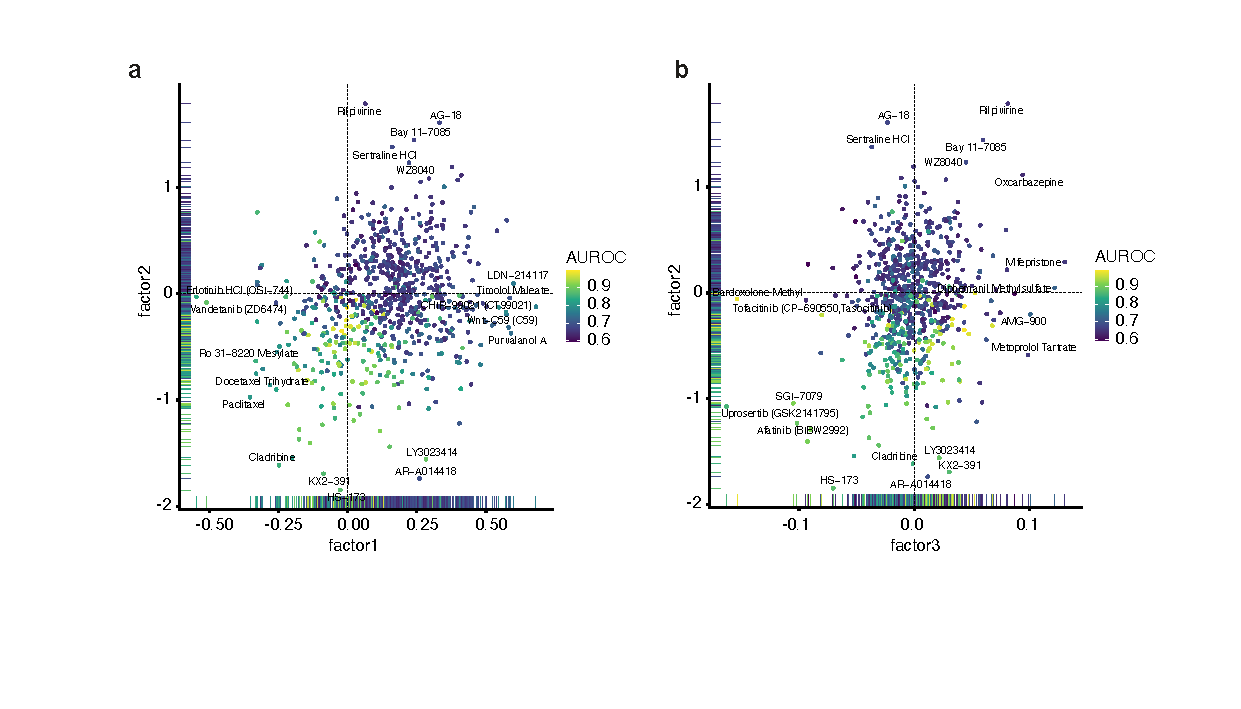
\includegraphics[width=\textwidth,
%                height=\textheight,
%                keepaspectratio]{figures/adenomaprofiling/pdf/fig_1_9.pdf}
%\caption{\textbf{Factor loadings for treatment activity. a} Factor 1 and 2 loadings, and \textbf{b} Factor 1 and 3 loadings. Average treatment activity score (AUROC) is color coded.}
%\label{fig_180}
%\end{figure}
%\bigbreak

\begin{figure}[h!]
\centering
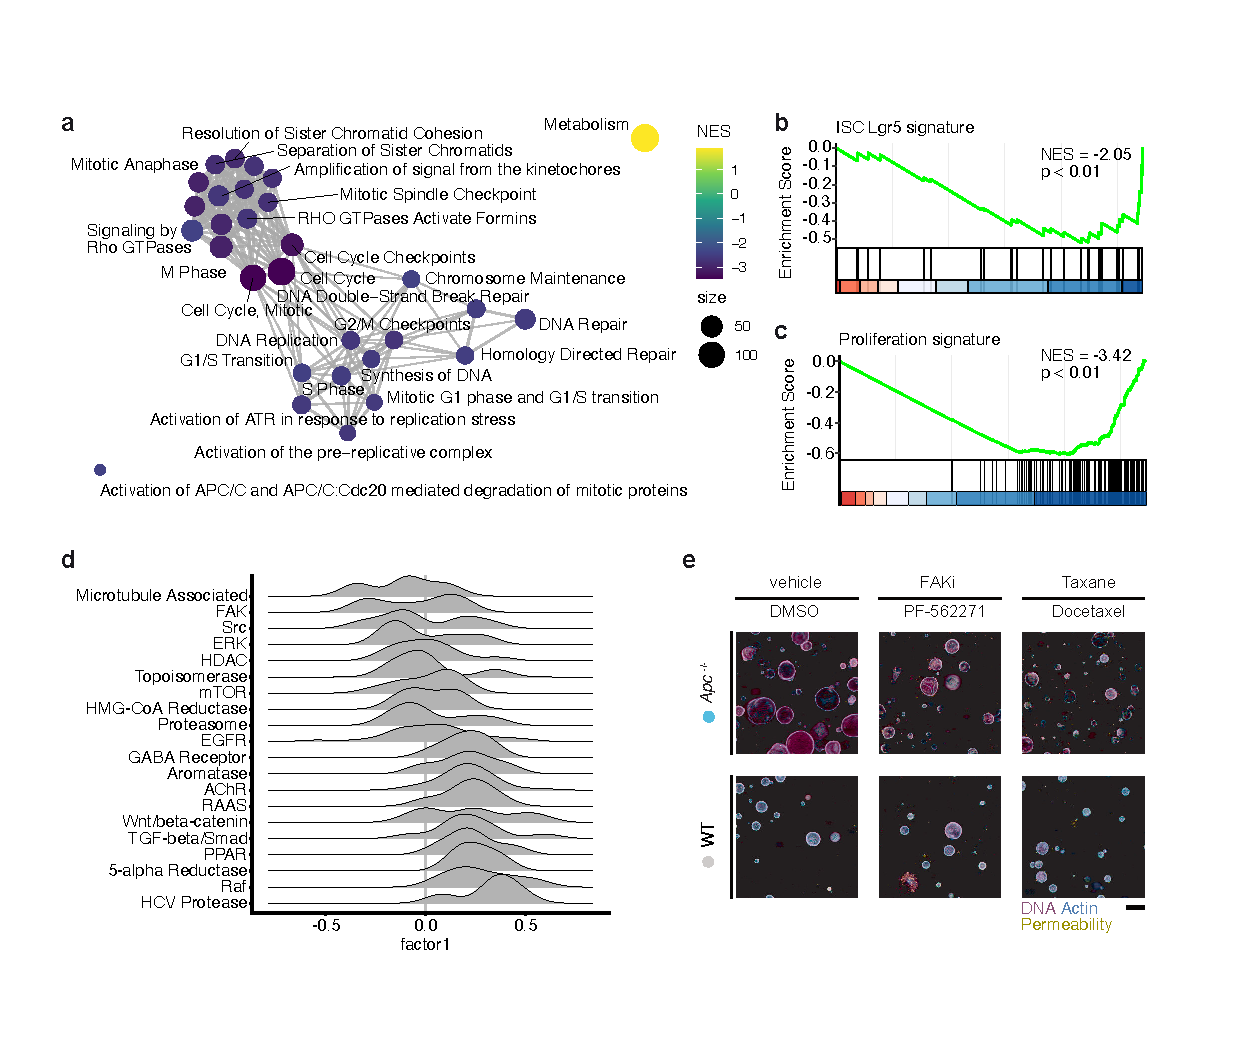
\includegraphics[width=\textwidth,
                height=\textheight,
                keepaspectratio]{figures/adenomaprofiling/pdf/fig_2_1.pdf}
\caption[Factor 1, canonical Wnt signaling]{\textbf{Factor 1, canonical Wnt signaling. a} Gene-set enrichment network of factor 1 gene expression loadings. An edge connects Reactome pathways with more than 20\% overlap. Central enriched processes include mitosis, DNA replication and DNA damage repair. \textbf{b and c} Gene set enrichment results of the "Lgr5 intestinal stem cell" and "proliferation" signature by Merlos-Suarez et al \citep{merlos-suarezIntestinalStemCell2011}. over ranked factor 1 gene expression loadings (ranking from high factor 1 loading to low factor 1 loading, NES = normalized enrichment score). \textbf{d} Distributions of treatment activity loadings grouped by drug target for factor 1. \textbf{e} Example images of compound treated organoids with WT or \textit{Apc}\textsuperscript{-/-}  genotype. Representaধve images are displayed (magenta = DNA, cyan = actin, yellow = cell permeability, scale-bar: 200μm).}
\label{fig_190}
\end{figure}
\bigbreak

Further exploration of the association between the treatment activity score and \textit{Apc} genotype showed that small molecule inhibitors of the canonical Wnt secretion pathway protein Porcupine (Porcn), IWP-L6 and LGK-974, were more active in \textit{Apc}\textsuperscript{+/+} organoids relative to their \textit{Apc}\textsuperscript{-/-}  counterparts \citep{liuTargetingWntdrivenCancer2013} (Figure \ref{fig_199}a). In contrast, this effect was not observable for PRI-724, a small molecule inhibitor targeting the interaction of beta-catenin and CREB-binding-protein in the canonical Wnt signaling pathway \citep{okazakiNovelInhibitorPRI7242019} (Figure \ref{fig_199}a). The observed differences in treatment activity scores among small molecule inhibitors are most likely related to their targets' relative location to Apc in the canonical Wnt signaling cascade. While Porcn-dependent Wnt secretion is generally upstream of the Apc-scaffolded destruction complex, the interaction of beta-catenin and the transcriptional coactivator CREB-binding-protein is located downstream of it. As a consequence, inhibition of destruction complex function by loss of \textit{Apc} is expected to render cells less sensitive to perturbations of the Wnt secretion cascade than direct perturbations of transcription factor binding properties (Figure \ref{fig_199}b).

\begin{figure}[h!]
\centering
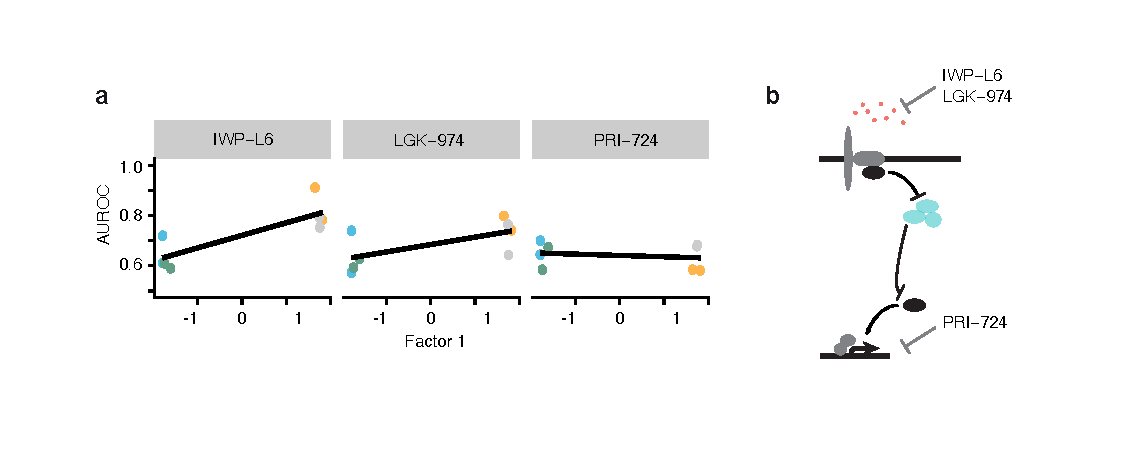
\includegraphics[scale=0.75,keepaspectratio]{figures/adenomaprofiling/pdf/fig_2_2_1.pdf}
\caption[Activity of small molecule Wnt signaling inhibitors]{\textbf{Activity of small molecule Wnt signaling inhibitors. a} AUROC activity score for three small molecule inhibitors of canonical Wnt signaling. \textbf{b} Target proteins for small molecules within the canonical Wnt signaling cascade with their relative position to the destruction complex (highlighted in blue).}
\label{fig_199}
\end{figure}
\bigbreak

\newpage

\subsection{A program caused by isolated \textit{Kras}\textsuperscript{G12D} activation shares signs of oncogene-induced senescence}
While the \textit{Apc}\textsuperscript{-/-}  genotype contributed primarily to factor 1 (Figure \ref{fig_180} b), the \textit{Kras}\textsuperscript{G12D} allele showed a strong loading for both factor 2 and factor 3. This observation corresponded with the fact that only organoid models without \textit{Apc} loss of function were separated by factor 2 (Figure \ref{fig_170} c). Factor 2 described a \textit{Kras}\textsuperscript{G12D} dependent change in cell state in the presence of intact \textit{Apc} function.


\begin{figure}[h!]
\centering
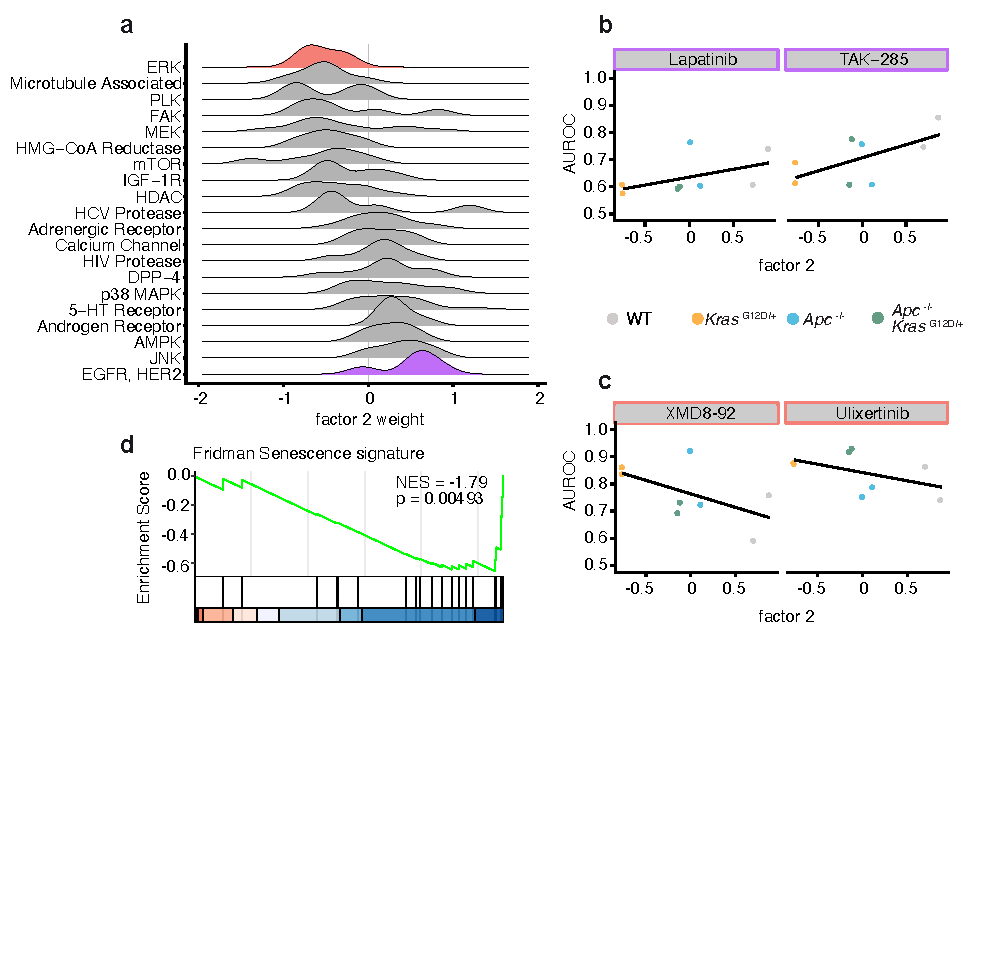
\includegraphics[scale=0.75,
                keepaspectratio]{figures/adenomaprofiling/pdf/fig_3_1_2.pdf}
\caption[Factor 2, isolated \textit{Kras}\textsuperscript{G12D} activity and oncogene induced senescence]{\textbf{Factor 2, isolated \textit{Kras}\textsuperscript{G12D} activity and oncogene induced senescence. a} Distributions of treatment activity loadings grouped by drug target for factor 2. \textbf{b} Relationship of representative ERK inhibitor activity with factor 2 score. Shown are compounds from highlighted groups in panel (a). \textbf{c} Relationship of representative EGFR inhibitor activity with factor 2 score. Shown are compounds from highlighted groups in panel (a). \textbf{d} Gene set enrichment results of a senescence signature \citep{fridmanCriticalPathwaysCellular2008} over ranked factor 2 gene expression loadings (ranking from high factor 2 loading to low factor 2 loading, NES = normalized enrichment score).}
\label{fig_200}
\end{figure}

As above, to understand the molecular mechanisms represented by factor 2, features with large absolute loadings were identified. ERK and MEK inhibitors were more active in factor 2 low models (\textit{Kras}\textsuperscript{G12D}+/-) while EGFR/HER2 inhibitors were more active in factor 2 high organoids (WT, figure \ref{fig_200} a and b). This juxtaposition in treatment activity against ERK-MAPK pathway members was reminiscent of the previous observations made for canonical Wnt signaling inhibitors (Figure \ref{fig_199}). With oncogenic \textit{Kras} localized between the receptor-layer (including Egfr and Her2) and downstream mediating kinases (for example Erk), hyperactive \textit{Kras} signaling likely leads to a cell state with relative resistance to EGFR inhibitors and increased dependency on Erk signaling. The previously observed transcriptional process of \textit{Egfr}-downregulation as a response to \textit{Kras}\textsuperscript{G12D}+/- is in line with these observations (Figure \ref{fig_162}b). 

\bigbreak

Oncogene induced senescence is a cell state marked by an arrest of the cell cycle and expression of pro-inflammatory mediators as a response to an oncogenic perturbation. An activated \textit{Kras}\textsuperscript{G12D}+/- genotype leads to oncogene induced senescence of colon epithelial cells in vivo \citepp{Bennecke2010-zf}. Prompted by previous reports on the effect of an isolated oncogenic \textit{Kras} allele, I identified an enrichment of a senescence related gene expression signature by Fridman et al. within the loadings of factor 2 \citep{fridmanCriticalPathwaysCellular2008} (Figure \ref{fig_200} c). Transcripts linked to cell senescence, including Igfbp3 (factor 2 loading ca. -0.999) and Hmga2 (factor 2 loading ca. -1.050) ranked among the strongest contributors to the factor. 
\bigbreak


\newpage
\subsection{A program describing the effect of oncogenic \textit{Kras} in the context of \textit{Apc} loss of function is marked by increased mTOR signaling }

While factor 2 captured the effect of oncogenic \textit{Kras} in an \textit{Apc} wildtype state, factor 3 scores separated organoid models by \textit{Kras} genotype in the context of an \textit{Apc} loss of function (Figure \ref{fig_170} c). On average, factor 3 only accounted for less than 10\% of variance across modalities within the MOFA model, supporting the overall similarity of \textit{Apc}\textsuperscript{-/-}  and Apc-/- \textit{Kras}\textsuperscript{G12D}+/- organoids previously observed separately on the transcriptome, proteome, lipidome and morphology level (Figure \ref{fig_161}a-d and \ref{fig_140} b).

\begin{figure}[h]
\centering
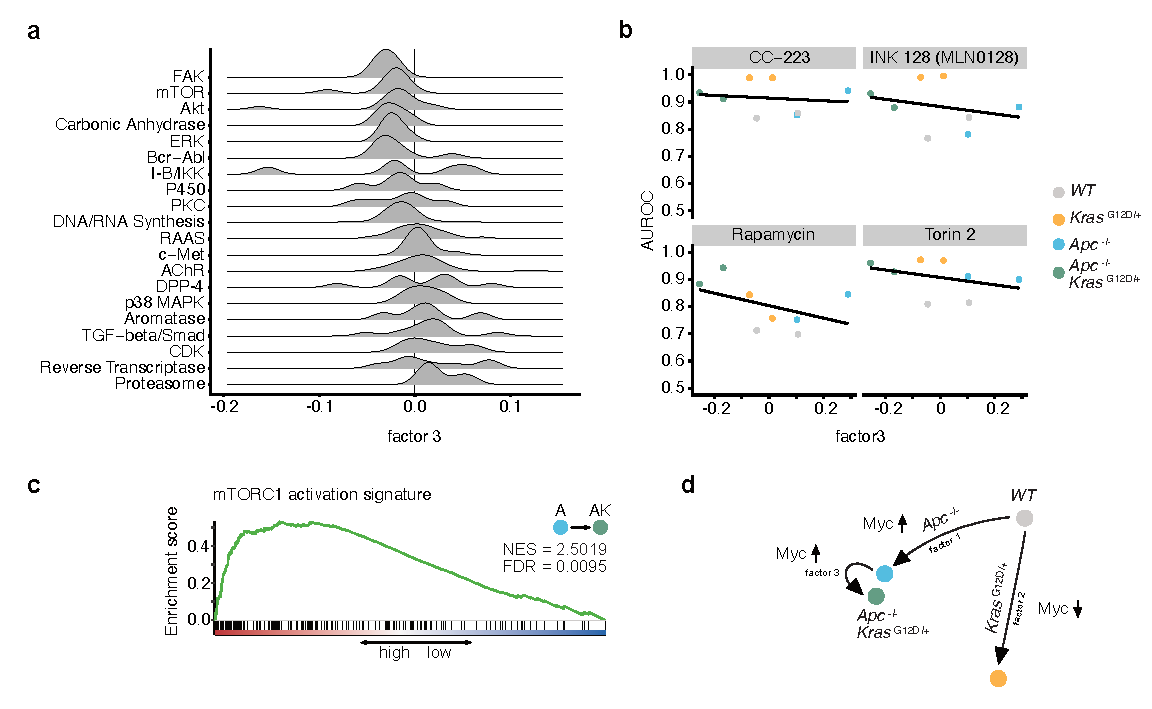
\includegraphics[scale=0.75,
                keepaspectratio]{figures/adenomaprofiling/pdf/fig_4_1.pdf}
\caption[Factor 3, \textit{Kras}\textsuperscript{G12D} effects in the context of \textit{Apc} loss of function]{\textbf{Factor 3, \textit{Kras}\textsuperscript{G12D} effects in the context of \textit{Apc} loss of function. a} Distributions of treatment activity loadings grouped by drug target for factor 3. \textbf{b} Relationship of representative mTOR inhibitor activity with factor 3 score. \textbf{c} Gene set enrichment results of a Reactome mTORC1 activation signature over ranked factor 3 gene expression loadings (ranking from high factor 3 loading to low factor 3 loading, NES = normalized enrichment score). \textbf{d} Visual summary of Myc gene set enrichment results for organoid state transitions. Myc signatures were significantly enriched in \textit{Apc}\textsuperscript{-/-}  models and depleted in models with isolated \textit{Kras}\textsuperscript{G12D}+/- mutation.}
\label{fig_300}
\end{figure}
\bigbreak

Exploration of factor 3 loadings identified mTOR and FAK inhibitor activity to contribute to a negative factor score. Double-mutant organoid models (Apc-/- \textit{Kras}\textsuperscript{G12D}+/-), which had a low factor 3 score, showed a greater treatment activity for these small molecule inhibitors than their single-mutant \textit{Apc}\textsuperscript{-/-}  counterparts (Figure \ref{fig_300} a). This difference in treatment activity was observerable for both ATP-competitive (e.g. INK-128, Sapanisertib) and non-ATP-competitive (e.g. Rapamycin) inhibitors (Figure \ref{fig_300} b). In line with the increased sensitvity to mTOR inhibitors, differential transcript expression analysis comparing single (Apc -/-, abbreviated A) and double mutant (Apc-/- \textit{Kras}\textsuperscript{G12D}+/-, abbreviated AK) organoids identified a significant increase in mTORC1 activation according to a Reactome signature (Figure \ref{fig_300} c, FDR=0.0095, NES=2.5019). In summary, factor 3 was aligned with the effect of oncogenic \textit{Kras} in \textit{Apc} mutant colon organoids and was characterized by increased transcriptional activity and sensitivity to mTOR signaling.


\newpage
\section{Interpreting treatment-induced organoid morphologies with Multi-omics factor analysis to identify small molecules with factor-specific effects}

To project the observed organoid morphologies (1699 treatments x 25 morphology features) into the previously learnt MOFA representation, the pseudoinverse of the morphology factor-weight matrix was approximated and factor scores were estimated (1699 treatments x 3 factors). Projection of treated organoid morphologies recovered the previously identified distribution of untreated organoid genotypes (Figure \ref{fig_500} c and d). As expected, treatments which showed a strong dispersion away from the centers formed by their respective genotype showed a high AUROC score (Figure \ref{fig_500} e and f).
\bigbreak

\begin{figure}[h]
\centering
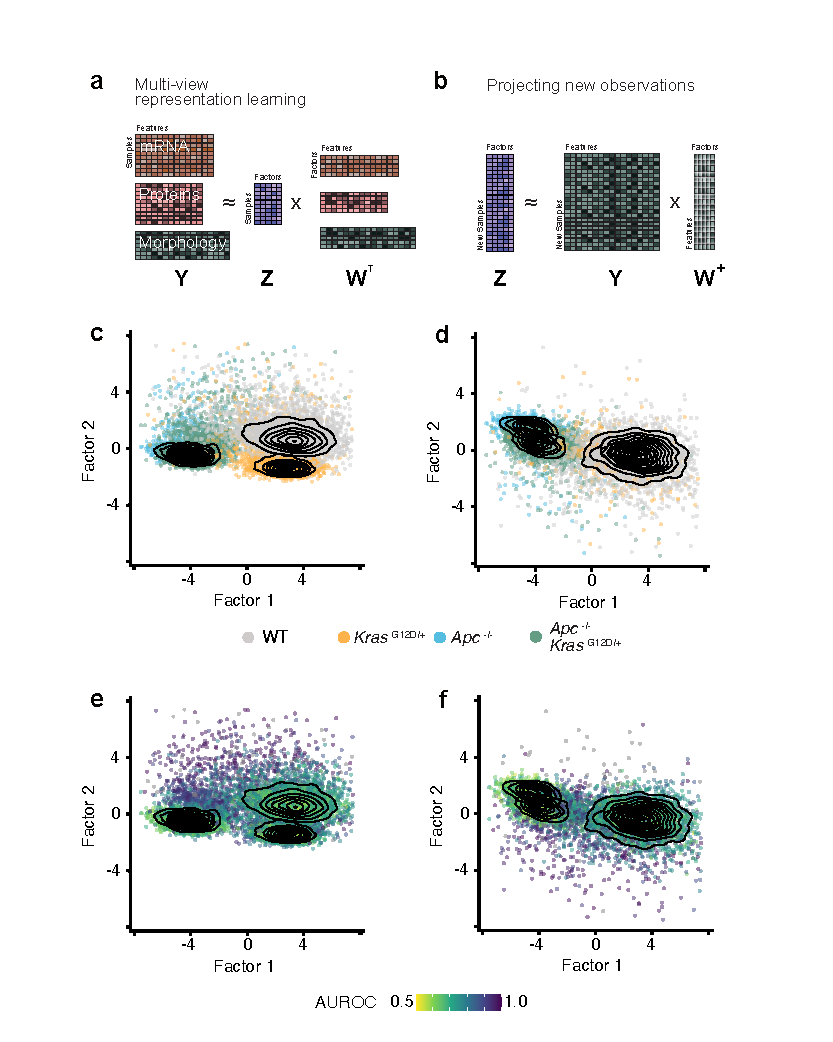
\includegraphics[scale=0.75,
                keepaspectratio]{figures/adenomaprofiling/pdf/fig_5_0.pdf}
\caption[Visualization of treated samples projected into factor space]{\textbf{Visualization of treated samples projected into factor space. a and b} Visualization of projected samples along factor 1, factor 2 and factor 3, respectively. Samples are colored by genotype. \textbf{c and d} Visualization of projected samples along factor 1, factor 2 and factor 3, respectively. Samples are colored by AUROC score distance from vehicle control (DMSO).}
\label{fig_500}
\end{figure}
\bigbreak


\begin{figure}[h]
\centering
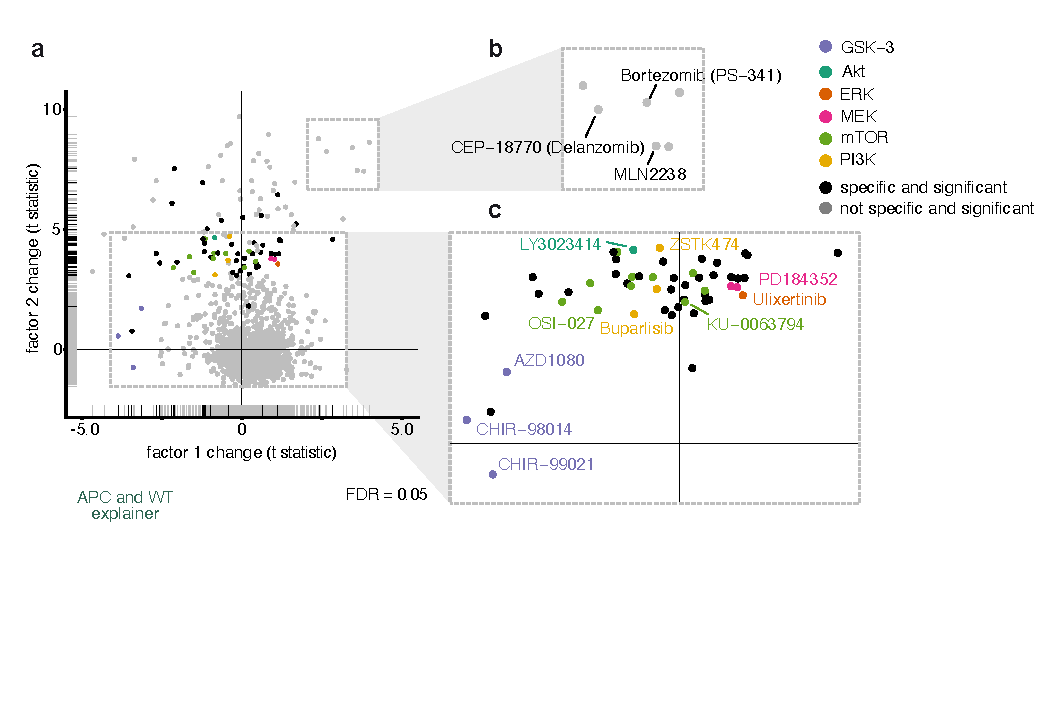
\includegraphics[scale=0.75,
                keepaspectratio]{figures/adenomaprofiling/pdf/fig_5_3_1.pdf}
\caption[Treatment-induced changes on factor 1 and factor 2 scores]{\textbf{Treatment-induced changes on factor 1 and factor 2 scores. a} Highlighted are treatments with a significant effect on projected scores for factor 1 and factor 2 across all organoid lines (ANOVA, FDR = 0.05). Treatments with a significant effect in only one of the three evaluated factors are highlighted in black. \textbf{b} Example for treatments with unspecific effects. Shown are Proteasome inhibitors. \textbf{c} Example for treatment with specific effects along one factor. Treatments are colored by their literature-derived mechanism of action.)}
\label{fig_180}
\end{figure}
\bigbreak

\subsection{Interpreting treatment-induced organoid morphologies using a learnt multi-omics factor model}

Next, I was interested in identifying treatments that changed organoid morphology along one of the two primary factors (Factors 1 and 2) that were previously identified. To this end an ANOVA modeling the factor scores as a function of the treatment and organoid line (without an interaction term) was performed for each factor (Figure \ref{fig_185} a). Of the x evaluated treatment, y ( \%) showed a significant effect on either factor 1 or factor 2, z showed an effect on both factors, and q showed no effect - thereby creating three groups: (1) treatments with a specific effect, (2) an unspecific effect, and (3) no observed effect. 
\par

As treatments that cause low-viability phenotypes, which were not modeled during training of the MOFA model, can cause spurious and unspecific effects in the learnt factor space, treatments with unspecific effects were inspected first. Among these treatments were multiple compounds which were tested at toxic concentrations including Proteasome inhibitors (i.e. Bortezomib; t =, Delanzomib; t= , Carfilzomib; t= ; Figure \ref{fig_185} b), conventional DNA-intercalating agents (i.e. Epirubicin; t=), and compounds with PAINS-like properties (Ellagic Acid; t=). 
\par

Among factor specific treatments, small molecules that displayed a negative effect on factor 1 (shifting from a state associated with an \textit{Apc} wildtype allele to an \textit{Apc}\textsuperscript{-/-}  associated state) were enriched for GSK3 beta inhibitors (i.e. CHIR-98014, CHIR-99021, LY2090314). Along factor 2, small molecules targeting downstream mediators of ERK-MAPK signaling (i.e.  PD184352, Ulixertinib) and PI3K-AKT-mTOR signaling (i.e. Buparlisib, KU−0063794) had a positive effect (shifting from a state associated with \textit{Kras}\textsuperscript{G12D} +/- genotype to a \textit{Kras} wildtype associated state). No treatment with positive effect on factor 1, indicating a shift from an \textit{Apc}\textsuperscript{-/-}  associated state towards an \textit{Apc} wildtype state was identified. 

\subsection{GSK3 beta inhibitors move \textit{Apc} wildtype organoids specifically along a canonical Wnt signaling program}

GSK3 beta is a kinase with central function within the canonical Wnt signaling destruction complex \citep{stamos} and inhibition of GSK3 beta has been shown to lead to hyperactivation of canonical Wnt signaling \citep{Stambolic}. Based on the fact that Apc -/- organoids are "already" in a state of high canonical Wnt signaling, I hypothesized that GSK3 beta inhibition should lead to a larger observed effect along factor 1 in \textit{Apc}\textsuperscript{+/+} organoids than their \textit{Apc}\textsuperscript{-/-}  counterparts, a case of treatment-genotype interaction. 

\begin{figure}[h]
\centering
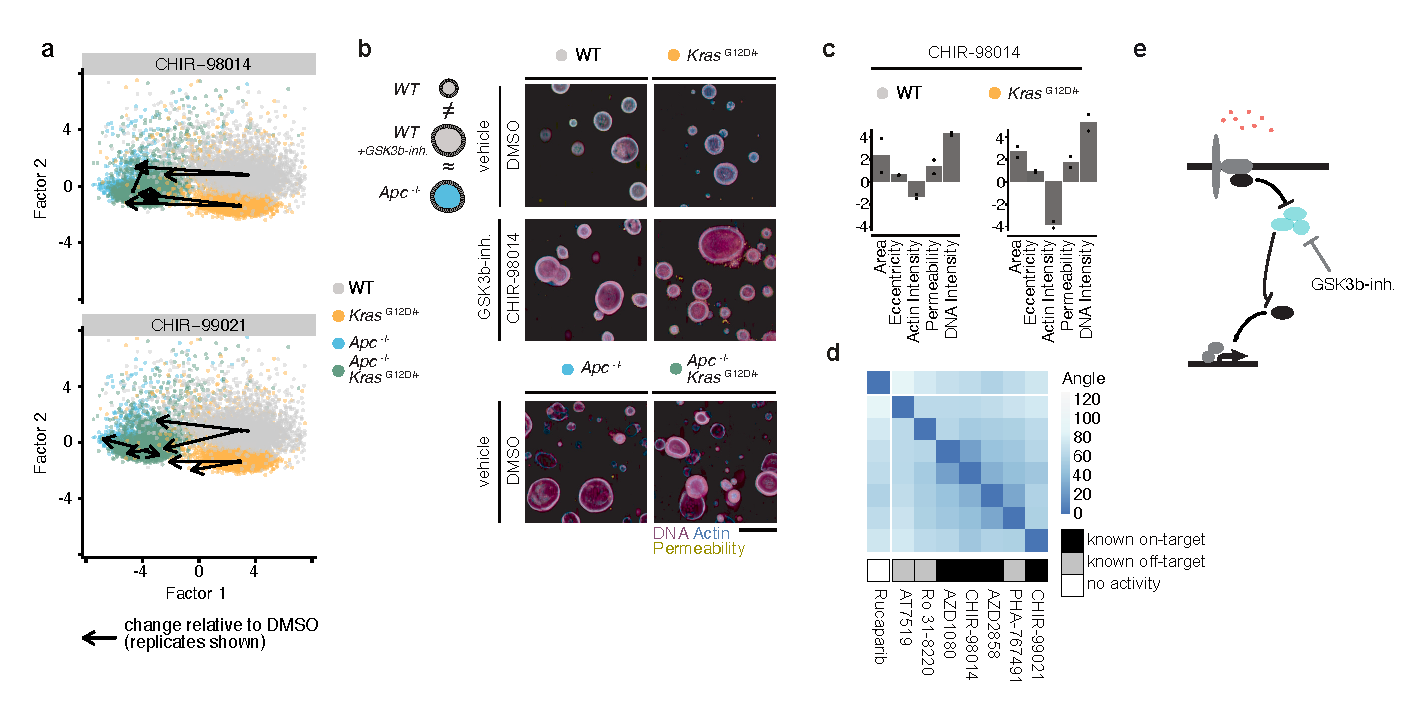
\includegraphics[scale=0.75,
                keepaspectratio]{figures/adenomaprofiling/pdf/fig_2_4_1.pdf}
\caption[GSK3 beta inhibition dependent morphology in colon organoid models]{\textbf{GSK3 beta inhibition dependent morphology in colon organoid models. a} Small molecule inhibition of GSK3 beta (CHIR98014) leads to phenocopying of \textit{Apc}\textsuperscript{-/-}  genotype organoid models. \textbf{b} Shift of morphological features of wildtype and \textit{Kras}\textsuperscript{G12D} +/- organoid models treated with CHIR98014. Shown is an increase in organoid size (Area) and DNA intensity. \textbf{c} Excerpt of clustering from figure \ref{fig_150} d, labeled with known binding activity of listed small molecules. Rucaparib is not member of the cluster and shown for comparison.}
\label{fig_185}
\end{figure}
\bigbreak

Indeed, the effect on factor 1 was stronger for WT and \textit{Kras}\textsuperscript{G12D}+/- organoid lines (Figure \ref{fig_185}). Treatment with the GSK3 beta inhibitor CHIR-98014 led to treatment-induced phenotypes in WT and \textit{Kras}\textsuperscript{G12D}+/- organoids that phenocopied the unperturbed morphology of \textit{Apc}\textsuperscript{-/-}  and double mutant organoid models (Figure \ref{fig_185} b). On the individual morphology feature level, treatment led to an increase in organoid size and DNA intensity (Figure \ref{fig_185} c) in \textit{Apc}\textsuperscript{+/+} models. This change in morphology was likely due to an increased proliferation rate of mutant cells, leading to rising organoid size and a higher density of nuclei per analyzed object. Guided by the identification of an interpretable GSK3 beta inhibition induced phenotype, I analyzed small molecules that clustered with known inhibitors of this kinase based on the similarity of their drug effect vectors (Figure \ref{fig_185} d). In line with the observations in this experiment, all small molecules clustering with well-described inhibitors of GSK3 beta had previously described off-target binding activity against this kinase within the LINCS KINOMEScan database \citep{subramanianNextGenerationConnectivity2017}. 
\par 

In summary, projecting treatment-induced morphologies into a factor space that was previously learnt from annotated organoid samples helped interpret small molecule effects and recovered previously known annotated on-target and off-target activity against GSK3 beta. In the future, I expect such an approach to assist in a iterative model-based exploration of complex in-vitro models by introducing structure-based treatment descriptors into the model and updating itl with new collected data at every experimental cycle.
\bigbreak

\end{flushleft}